%!TEX TS-program = xelatex
\documentclass[]{friggeri-cv}
\usepackage{afterpage}
\usepackage{wrapfig} %preámbulo
\usepackage{hyperref}
\usepackage{color}
\usepackage{xcolor}
\hypersetup{
    pdftitle={},
    pdfauthor={},
    pdfsubject={},
    pdfkeywords={},
    colorlinks=false,       % no lik border color
   allbordercolors=white    % white border color for all
}
\addbibresource{bibliography.bib}
\RequirePackage{xcolor}
\definecolor{pblue}{HTML}{0395DE}

\begin{document}

\header{Álvaro} {Camps} {Palou de Comasema}{Software Engineer}

      
% Fake text to add separator      
\fcolorbox{white}{gray}{\parbox{\dimexpr\textwidth-2\fboxsep-2\fboxrule}{%
.....
}}

% In the aside, each new line forces a line break
\begin{aside}
  \section{Dirreción}
    Paseo de la Estación, 9-5ºA
    28807, Alcalá de Henares, Madrid
    ~
  \section{Tel \& Skype}
    +34 686 88 99 52
    alvarocampspalou
    ~
  \section{eMail}
    \href{mailto:a.campspc@gmail.com}{\textbf{a.campspc@}\\gmail.com}
    ~
  \section{Web \& In}
    \href{http://campspalou.no-ip.biz}{campspalou.no-ip.biz}
    \href{https://es.linkedin.com/pub/alvaro-camps-palou-de-comasema/}{es.linkedin.com/pub/ alvaro-camps-palou-de-comasema/}
    ~
  \section{Programación}
    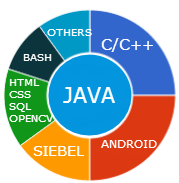
\includegraphics[scale=0.62]{img/programming.png}
    ~
  \section{Preferencias OS}
    \textbf{GNU/Linux}
\includegraphics[scale=0.40]{img/5stars.png}
    \textbf{Unix}
\includegraphics[scale=0.40]{img/4stars.png}
    \textbf{Windows}
\includegraphics[scale=0.40]{img/2stars.png}
    \textbf{MacOS}
\includegraphics[scale=0.40]{img/1stars.png}
    ~
  \section{Idiomas}
    \textbf{Español}
\includegraphics[scale=0.40]{img/5stars.png}
    \textbf{Inglés}
\includegraphics[scale=0.40]{img/3stars.png}
    ~
  \section{QR de contacto}
    
\includegraphics[scale=0.35]{img/QR.png}
    ~
\end{aside}

\section{Experiencia}
\begin{entrylist}
  \entry
    {12/13 - Actualidad}
    {Software Engineer, Programador}
    {Accenture Technology Solutions , Madrid, España}
    {Diseño y desarrollo de interfaces, pruebas de integracion y pruebas de 2a2 para el CRM Siebel 8 para el cliente Orange S.A \\}
    {Tecnologia: Siebel\\}
  \entry
    {03/12 - 01/12}
    {Becario fundación UAH,Programador Junior}
    {GRAM - Multisensorial Analysis and Recognition Group, Universidad de Alcalá de Henares}
    {Diseño y desarrollo la aplicación Sistema de Lector de Matriculas Embarcado (LME).\\}
    {Tegnologia: C/C++, Matrox Imaging Library, MySQL\\}
    \entry
    {01/11 - 31/11}
    {Becario UAH, becario de formación}
    {Universidad de Alcalá de Henares}
    {Las funciones realizadas en aulas de informática: resolver problemas con los ordenadores y sistemas operativos, prestar material, mantenimiento de software, cambios de configuración, etc. }
    {}

\end{entrylist}

\section{Educación}
\begin{entrylist}
  \entry
    {2013}
    {Ingeniería Técnica en Informática de Sistemas}
    {Universidad de Alcalá de Henares, Madrid}
    {Conocimientos técnicos: matemáticas, lógica, ingeniería, física y electrónica.\\
    \emph{Proyecto Final de Carrera: "Sistema De Reconocimiento De Objetos En Dispositivos Móviles Para Tratamiento De Trastornos Del Lenguaje".}\\
    \emph{El Proyecto Final de Carrera fue realizado para dispositivos móviles Android utilizando Java y C++.\\ \textbf{Nota}: Sobresaliente}.}
{}   
\end{entrylist}

\section{Formación complementaria}
\begin{entrylist}
\entry
    {2009}
    {Curso de seguridad}
    {Universidad de Alcalá de Henares}
    {Curso de Auditoría de Seguridad Informática por la Universidad de Alcalá de Henares}{}
   \entry
    {2009}
    {Curso de seguridad}
    {Universidad de Alcalá de Henares}
    {Curso Básico de Seguridad Informática por la Universidad de Alcalá de Henares}
{}   \entry
    {2009}
    {Curso de programación Java}
    {Accenture}
    {Programa de Formación en Entorno JAVA}
{}
\end{entrylist}


\section{Otros datos de interés}
\begin{entrylist}
\entry
    {}
    {Estancia de estudio en la escuela de inglés ISI English Language Schoolen Dublin, Irlanda.}
    {}{Autorización para la conducción de vehículos B.\\
    Disponibilidad para movilidad geográfica.}
    {}
\end{entrylist}



\end{document}
